% Options for packages loaded elsewhere
% Options for packages loaded elsewhere
\PassOptionsToPackage{unicode}{hyperref}
\PassOptionsToPackage{hyphens}{url}
%
\documentclass[
  ignorenonframetext,
]{beamer}
\newif\ifbibliography
\usepackage{pgfpages}
\setbeamertemplate{caption}[numbered]
\setbeamertemplate{caption label separator}{: }
\setbeamercolor{caption name}{fg=normal text.fg}
\beamertemplatenavigationsymbolsempty
% remove section numbering
\setbeamertemplate{part page}{
  \centering
  \begin{beamercolorbox}[sep=16pt,center]{part title}
    \usebeamerfont{part title}\insertpart\par
  \end{beamercolorbox}
}
\setbeamertemplate{section page}{
  \centering
  \begin{beamercolorbox}[sep=12pt,center]{section title}
    \usebeamerfont{section title}\insertsection\par
  \end{beamercolorbox}
}
\setbeamertemplate{subsection page}{
  \centering
  \begin{beamercolorbox}[sep=8pt,center]{subsection title}
    \usebeamerfont{subsection title}\insertsubsection\par
  \end{beamercolorbox}
}
% Prevent slide breaks in the middle of a paragraph
\widowpenalties 1 10000
\raggedbottom
\AtBeginPart{
  \frame{\partpage}
}
\AtBeginSection{
  \ifbibliography
  \else
    \frame{\sectionpage}
  \fi
}
\AtBeginSubsection{
  \frame{\subsectionpage}
}
\usepackage{iftex}
\ifPDFTeX
  \usepackage[T1]{fontenc}
  \usepackage[utf8]{inputenc}
  \usepackage{textcomp} % provide euro and other symbols
\else % if luatex or xetex
  \usepackage{unicode-math} % this also loads fontspec
  \defaultfontfeatures{Scale=MatchLowercase}
  \defaultfontfeatures[\rmfamily]{Ligatures=TeX,Scale=1}
\fi
\usepackage{lmodern}

\ifPDFTeX\else
  % xetex/luatex font selection
\fi
% Use upquote if available, for straight quotes in verbatim environments
\IfFileExists{upquote.sty}{\usepackage{upquote}}{}
\IfFileExists{microtype.sty}{% use microtype if available
  \usepackage[]{microtype}
  \UseMicrotypeSet[protrusion]{basicmath} % disable protrusion for tt fonts
}{}
\makeatletter
\@ifundefined{KOMAClassName}{% if non-KOMA class
  \IfFileExists{parskip.sty}{%
    \usepackage{parskip}
  }{% else
    \setlength{\parindent}{0pt}
    \setlength{\parskip}{6pt plus 2pt minus 1pt}}
}{% if KOMA class
  \KOMAoptions{parskip=half}}
\makeatother


\usepackage{longtable,booktabs,array}
\usepackage{calc} % for calculating minipage widths
\usepackage{caption}
% Make caption package work with longtable
\makeatletter
\def\fnum@table{\tablename~\thetable}
\makeatother
\usepackage{graphicx}
\makeatletter
\newsavebox\pandoc@box
\newcommand*\pandocbounded[1]{% scales image to fit in text height/width
  \sbox\pandoc@box{#1}%
  \Gscale@div\@tempa{\textheight}{\dimexpr\ht\pandoc@box+\dp\pandoc@box\relax}%
  \Gscale@div\@tempb{\linewidth}{\wd\pandoc@box}%
  \ifdim\@tempb\p@<\@tempa\p@\let\@tempa\@tempb\fi% select the smaller of both
  \ifdim\@tempa\p@<\p@\scalebox{\@tempa}{\usebox\pandoc@box}%
  \else\usebox{\pandoc@box}%
  \fi%
}
% Set default figure placement to htbp
\def\fps@figure{htbp}
\makeatother





\setlength{\emergencystretch}{3em} % prevent overfull lines

\providecommand{\tightlist}{%
  \setlength{\itemsep}{0pt}\setlength{\parskip}{0pt}}



 


\makeatletter
\@ifpackageloaded{caption}{}{\usepackage{caption}}
\AtBeginDocument{%
\ifdefined\contentsname
  \renewcommand*\contentsname{Table of contents}
\else
  \newcommand\contentsname{Table of contents}
\fi
\ifdefined\listfigurename
  \renewcommand*\listfigurename{List of Figures}
\else
  \newcommand\listfigurename{List of Figures}
\fi
\ifdefined\listtablename
  \renewcommand*\listtablename{List of Tables}
\else
  \newcommand\listtablename{List of Tables}
\fi
\ifdefined\figurename
  \renewcommand*\figurename{Figure}
\else
  \newcommand\figurename{Figure}
\fi
\ifdefined\tablename
  \renewcommand*\tablename{Table}
\else
  \newcommand\tablename{Table}
\fi
}
\@ifpackageloaded{float}{}{\usepackage{float}}
\floatstyle{ruled}
\@ifundefined{c@chapter}{\newfloat{codelisting}{h}{lop}}{\newfloat{codelisting}{h}{lop}[chapter]}
\floatname{codelisting}{Listing}
\newcommand*\listoflistings{\listof{codelisting}{List of Listings}}
\makeatother
\makeatletter
\makeatother
\makeatletter
\@ifpackageloaded{caption}{}{\usepackage{caption}}
\@ifpackageloaded{subcaption}{}{\usepackage{subcaption}}
\makeatother

\usepackage{bookmark}
\IfFileExists{xurl.sty}{\usepackage{xurl}}{} % add URL line breaks if available
\urlstyle{same}
\hypersetup{
  pdftitle={Week 5},
  pdfauthor={Jonathan A. Pedroza (JP) PhD},
  hidelinks,
  pdfcreator={LaTeX via pandoc}}


\title{Week 5}
\subtitle{Literature Review}
\author{Jonathan A. Pedroza (JP) PhD}
\date{2026-09-12}

\begin{document}
\frame{\titlepage}


\begin{frame}{Today's Icebreaker}
\phantomsection\label{todays-icebreaker}
\begin{itemize}
\tightlist
\item
  If you've met with your potential advisor(s), how has your original
  idea changed?

  \begin{itemize}
  \tightlist
  \item
    If you haven't met with them, what field of research are you
    thinking of looking at to match research from your potential
    advisor(s)?
  \end{itemize}
\item
  What are some keywords that come to mind when thinking about your
  research topic?
\end{itemize}
\end{frame}

\begin{frame}{JP's Response}
\phantomsection\label{jps-response}
\begin{itemize}
\tightlist
\item
  Additional focal points

  \begin{itemize}
  \tightlist
  \item
    No longer focused on intervention design and now focused on
    prediction
  \item
    Thinking through pros and cons of interviews vs focus groups
  \end{itemize}
\item
  Keywords include:

  \begin{itemize}
  \tightlist
  \item
    Mathematics
  \item
    Self-efficacy OR self efficacy
  \item
    Grades
  \item
    College OR university OR higher education
  \item
    Cluster
  \end{itemize}
\end{itemize}
\end{frame}

\begin{frame}{How to Look for Articles}
\phantomsection\label{how-to-look-for-articles}
\begin{itemize}
\item
  Use keywords
\item
  Don't type out full statements
\item
  Use forward \& backward searches
\item
  AI Options
\end{itemize}
\end{frame}

\begin{frame}{How to Look for Articles}
\phantomsection\label{how-to-look-for-articles-1}
\begin{itemize}
\item
  \href{https://scholar.google.com/}{Google Scholar}
\item
  Can use the \href{https://www.lib.berkeley.edu/}{Berkeley Library
  website}
\end{itemize}
\end{frame}

\begin{frame}{Connect Google Scholar to UCB Library}
\phantomsection\label{connect-google-scholar-to-ucb-library}
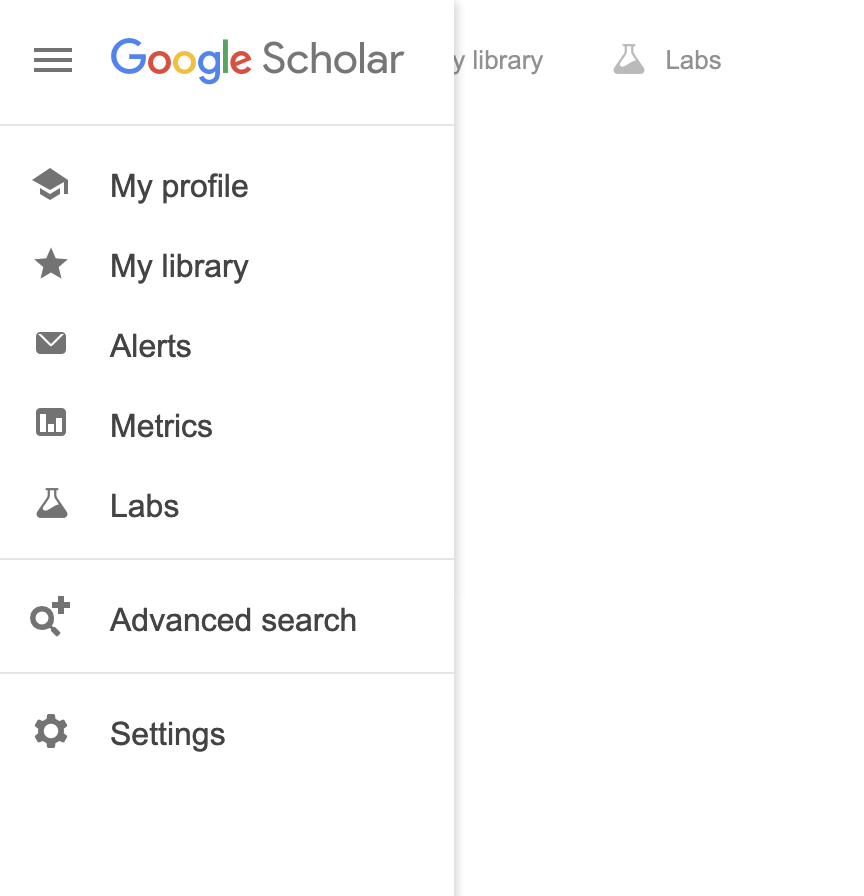
\includegraphics[width=0.6\linewidth,height=\textheight,keepaspectratio]{settings.png}
\end{frame}

\begin{frame}{Connect Google Scholar to UCB Library}
\phantomsection\label{connect-google-scholar-to-ucb-library-1}
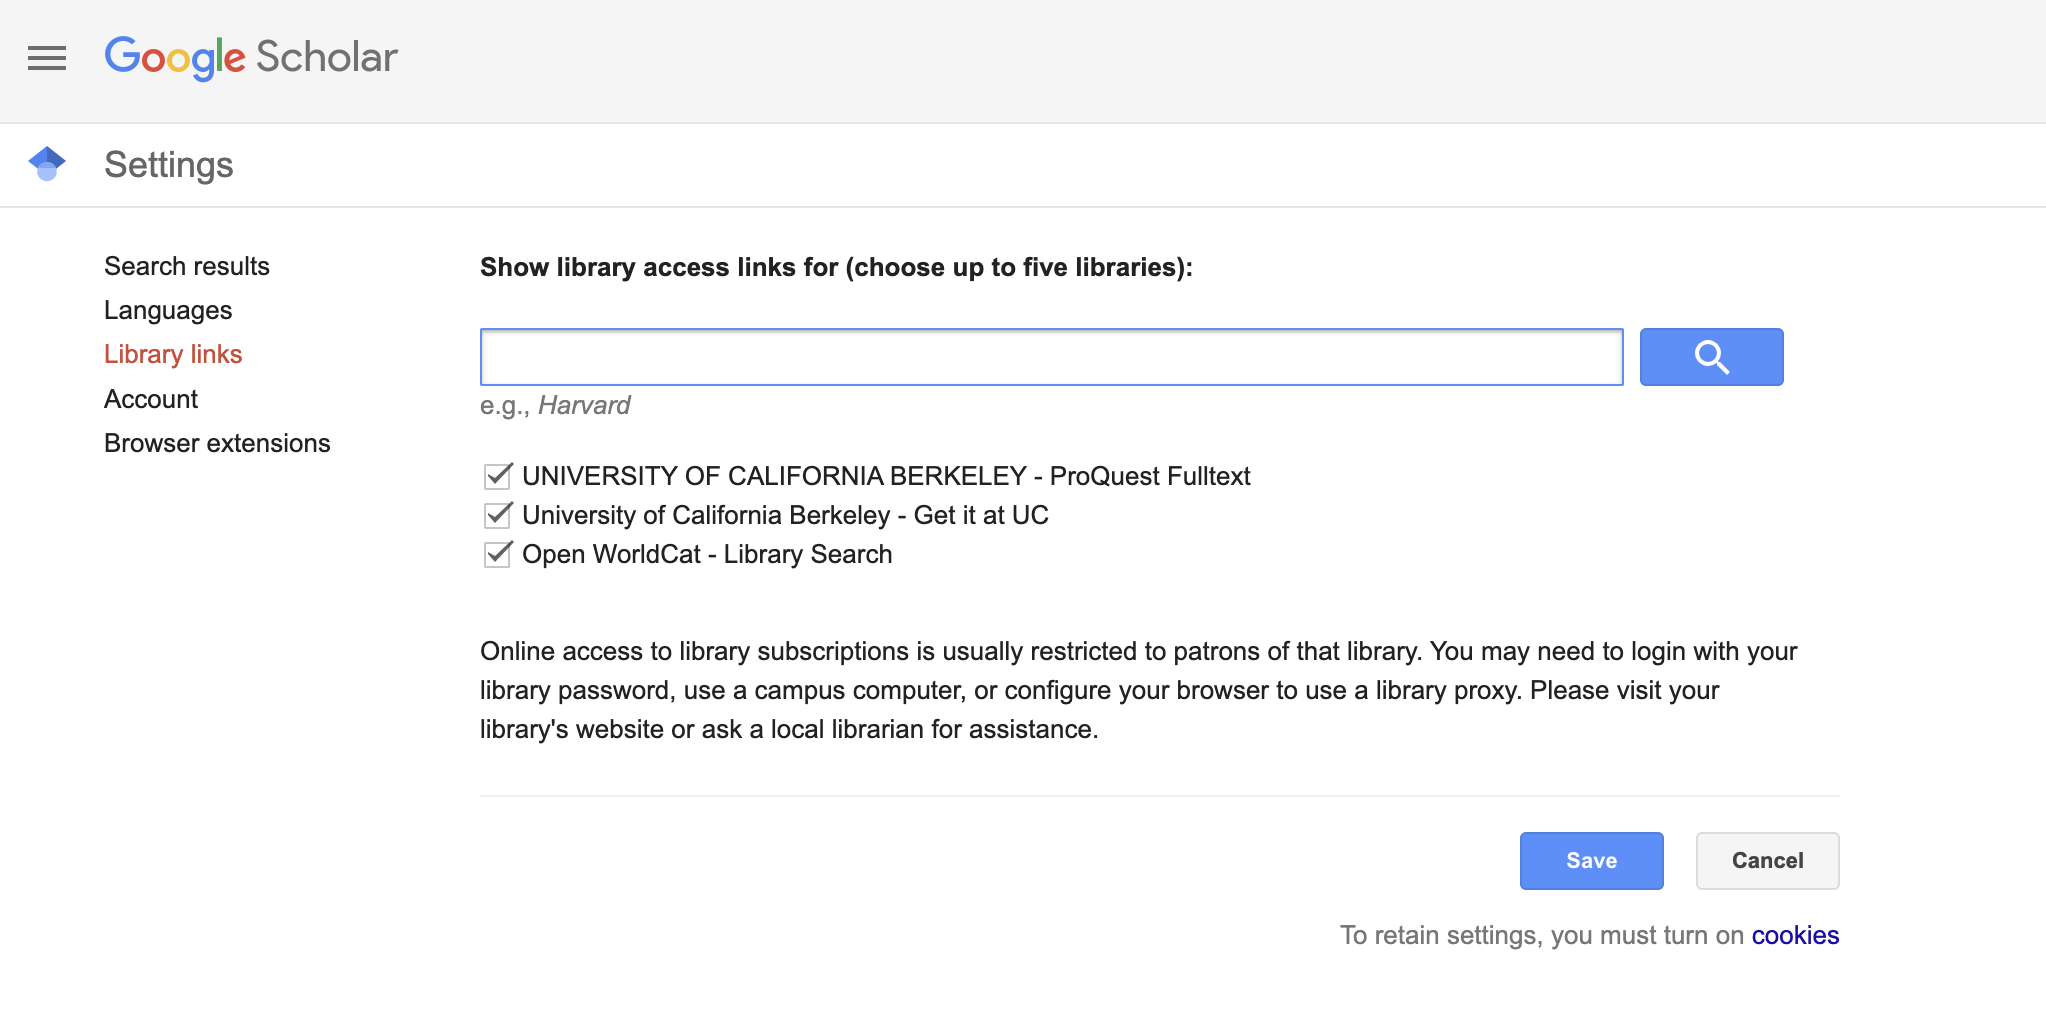
\includegraphics[width=0.6\linewidth,height=\textheight,keepaspectratio]{ucb_library.png}
\end{frame}

\begin{frame}[fragile]{Keywords}
\phantomsection\label{keywords}
\begin{itemize}
\tightlist
\item
  Use \texttt{AND}, \texttt{OR}, \texttt{()}, \texttt{-}, \texttt{""},
  \texttt{\textasciitilde{}}, \texttt{*}

  \begin{itemize}
  \tightlist
  \item
    Artificial Intelligence OR AI
  \item
    Artificial Intelligence AND Learning
  \item
    (Artificial Intelligence OR AI) AND Learning
  \item
    (Artificial Intelligence OR AI) AND Learning AND -Deep (- = don't
    include)
  \item
    (``Artificial Intelligence'' OR AI) AND Learning AND -``Deep
    Learning'' (``\,'' = Look up exact term)
  \item
    (``Artificial Intelligence'' OR AI) AND (Learning OR
    \textasciitilde education) AND -``Deep Learning'' (\textasciitilde{}
    = Look up synonyms)
  \item
    (``Artificial Intelligence'' OR AI) AND ((Learning OR educat\emph{)
    AND (college OR university OR ``higher education'')) AND -``Deep
    Learning'' (} = Any word with the same beginning)
  \end{itemize}
\end{itemize}
\end{frame}

\begin{frame}{Keywords}
\phantomsection\label{keywords-1}
\begin{itemize}
\tightlist
\item
  Sometimes your searches can sound problematic

  \begin{itemize}
  \tightlist
  \item
    Example: (Latina OR Latino OR Latinx OR Latine OR Hispanic OR
    \emph{Mexican})
  \item
    Why not Latin*?
  \end{itemize}
\item
  \href{https://library.acg.edu/how-to-guides/google-scholar/advanced-searching}{Resource
  here}
\end{itemize}
\end{frame}

\begin{frame}{Forward Searches}
\phantomsection\label{forward-searches}
\begin{itemize}
\tightlist
\item
  You find an amazing article

  \begin{itemize}
  \tightlist
  \item
    Maybe it is too old
  \item
    Has useful information
  \end{itemize}
\item
  Look at who cites that paper

  \begin{itemize}
  \tightlist
  \item
    Re-use your keywords in this new search
  \end{itemize}
\end{itemize}
\end{frame}

\begin{frame}{Example of Forward Search}
\phantomsection\label{example-of-forward-search}
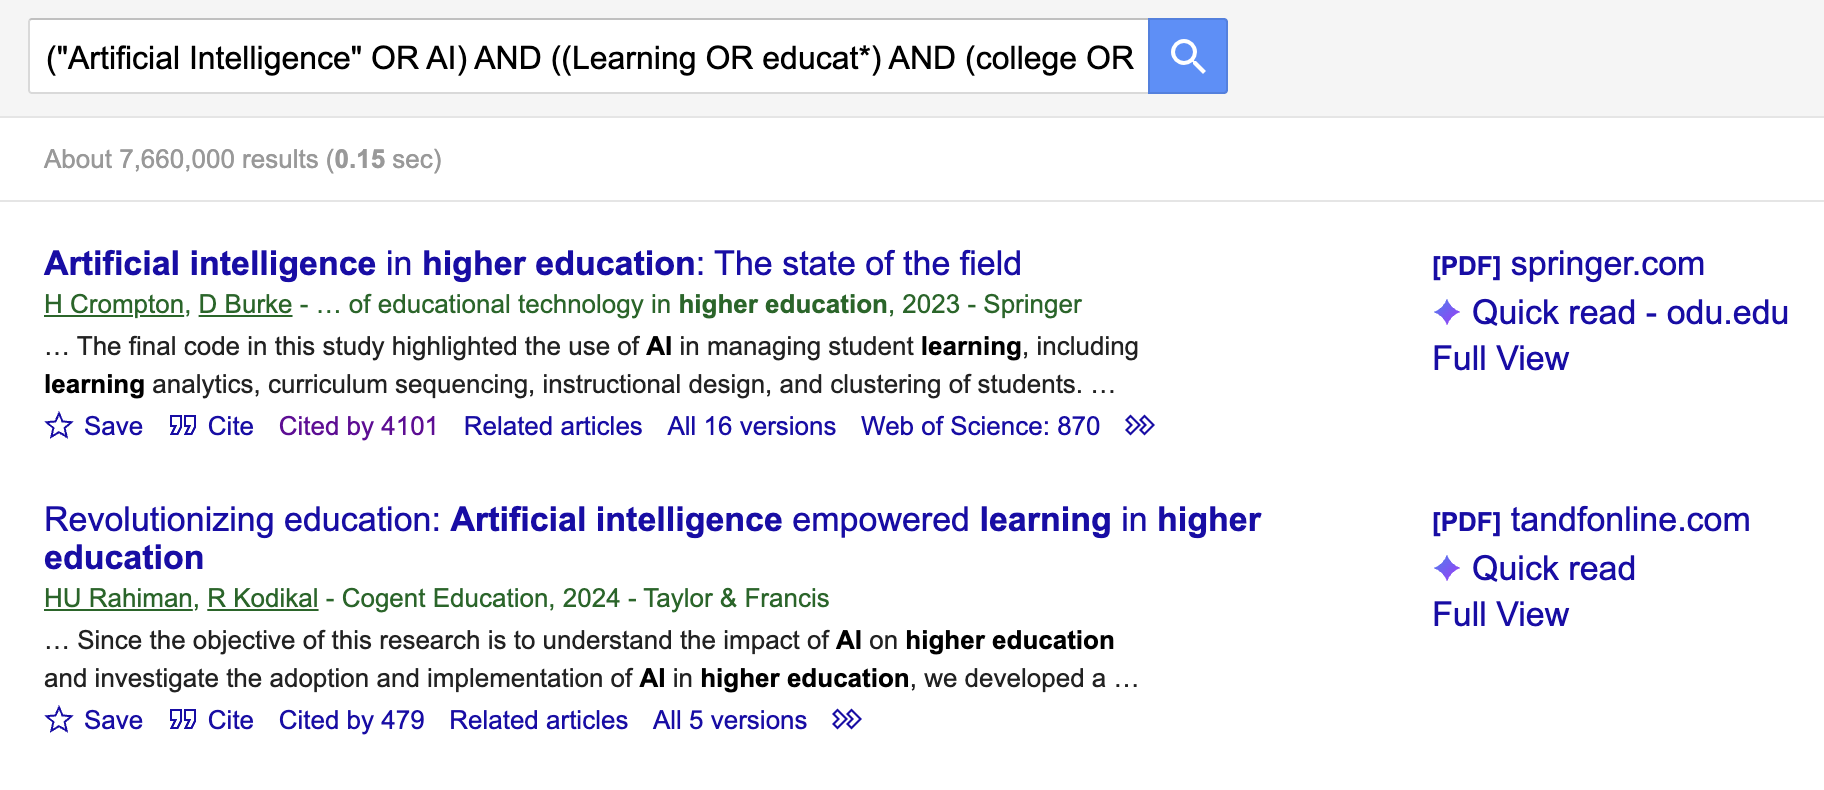
\includegraphics[width=0.6\linewidth,height=\textheight,keepaspectratio]{article.png}
\end{frame}

\begin{frame}{Example of Forward Search}
\phantomsection\label{example-of-forward-search-1}
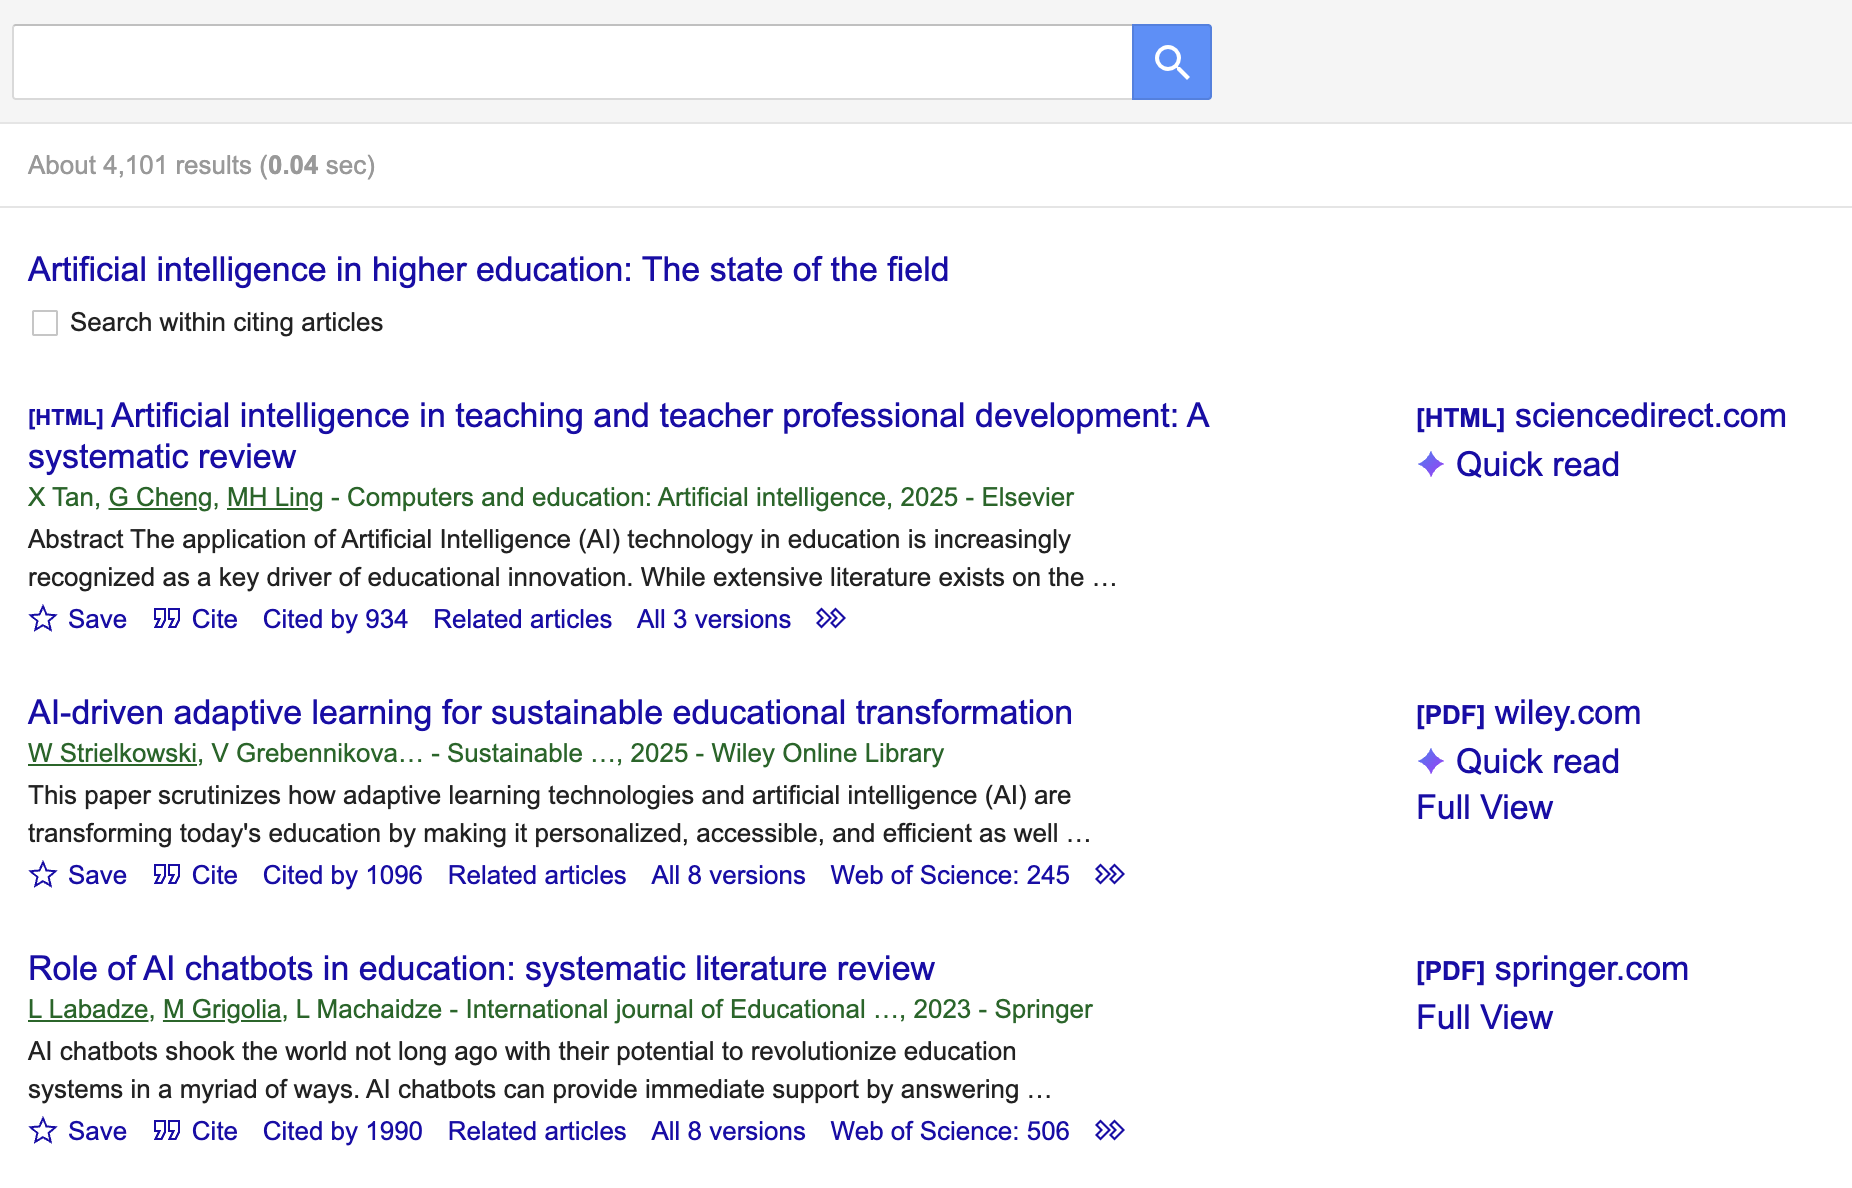
\includegraphics[width=0.6\linewidth,height=\textheight,keepaspectratio]{forward.png}
\end{frame}

\begin{frame}{Example of Forward Search}
\phantomsection\label{example-of-forward-search-2}
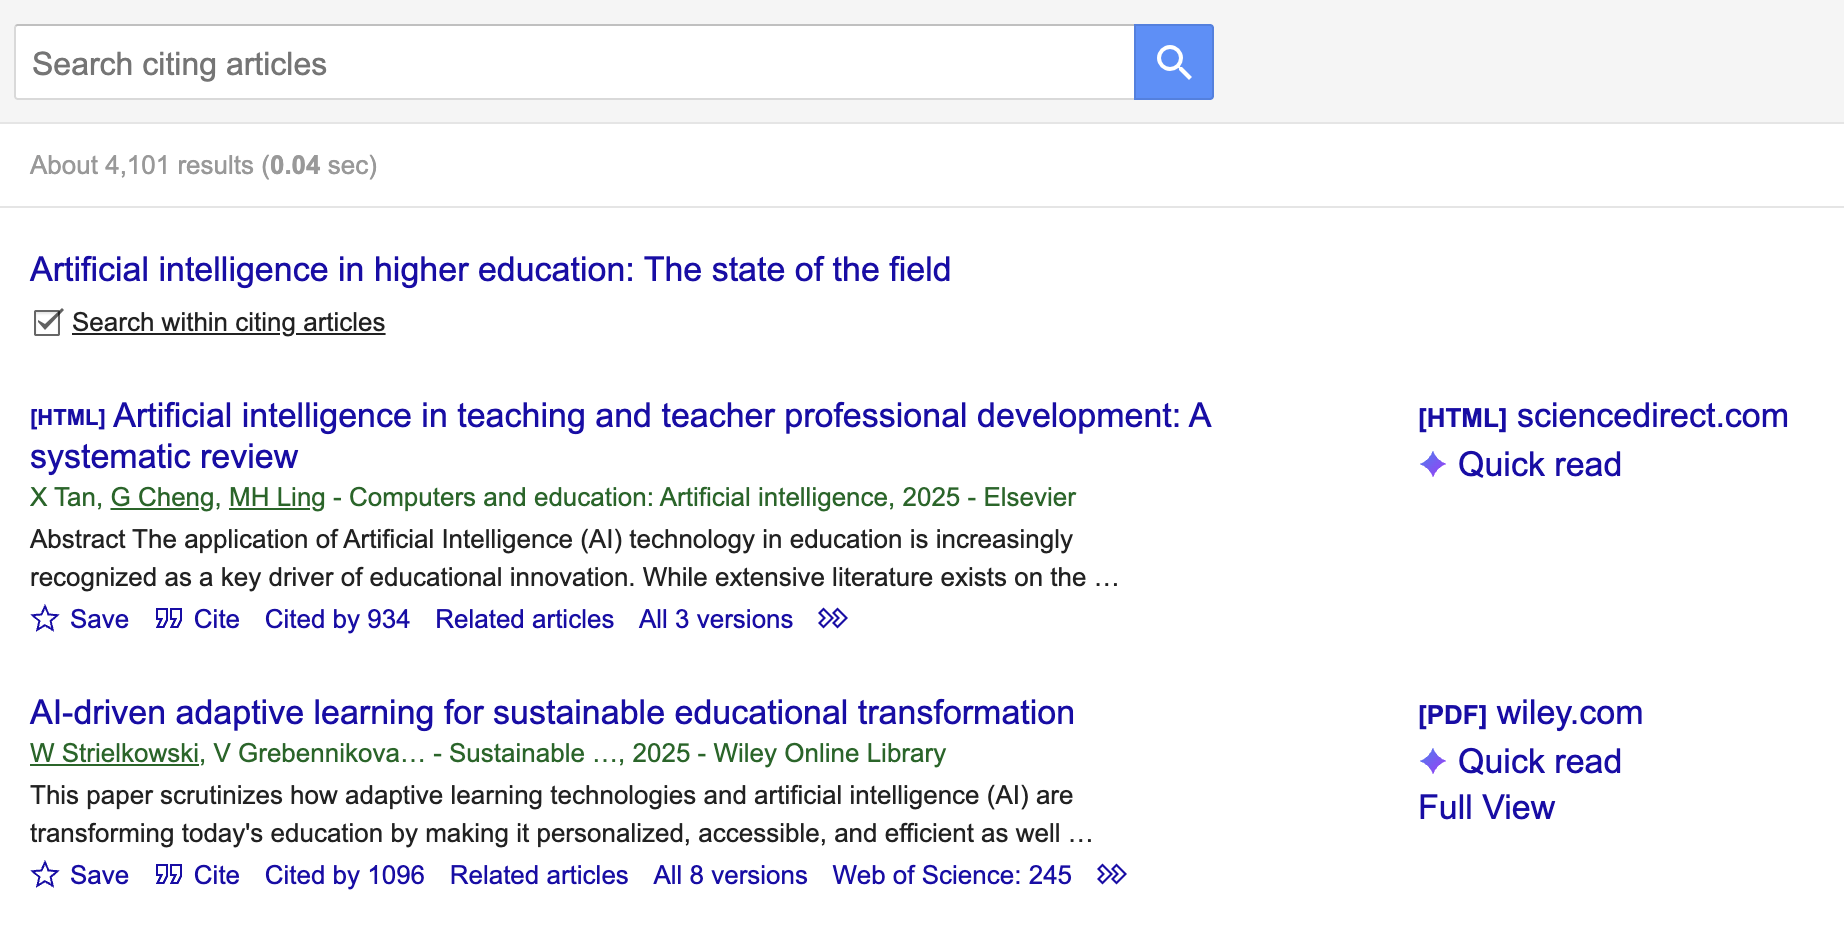
\includegraphics[width=0.6\linewidth,height=\textheight,keepaspectratio]{forward2.png}
\end{frame}

\begin{frame}{Example of Forward Search}
\phantomsection\label{example-of-forward-search-3}
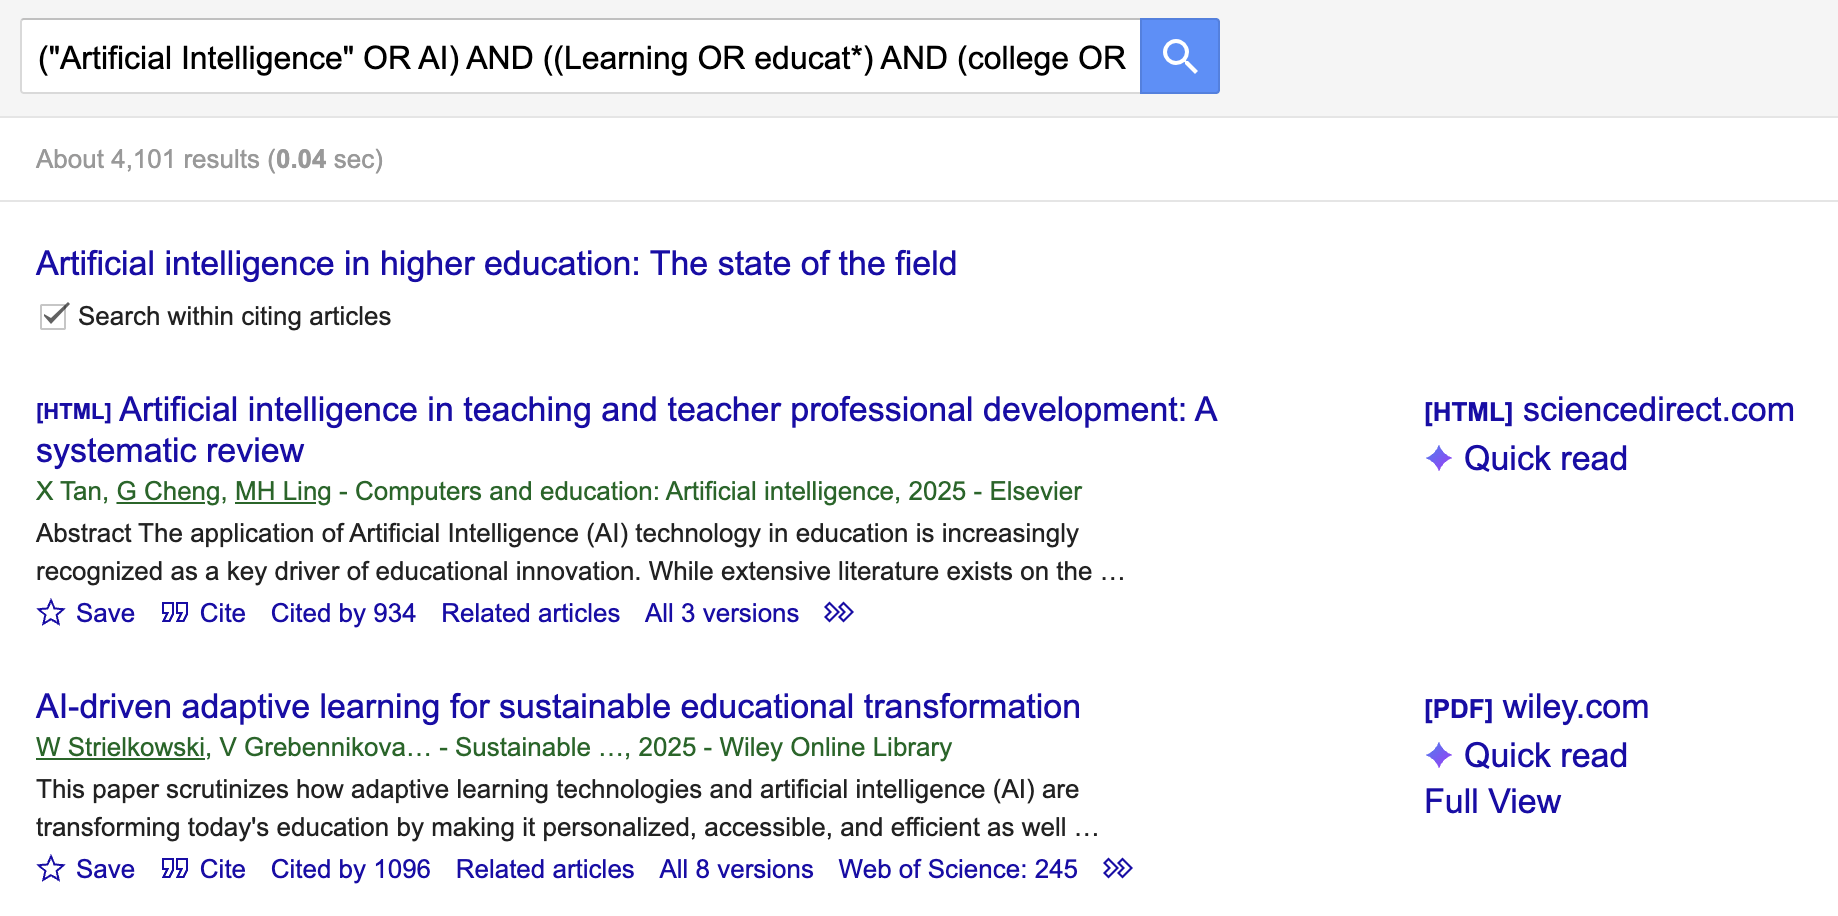
\includegraphics[width=0.6\linewidth,height=\textheight,keepaspectratio]{bring_search.png}
\end{frame}

\begin{frame}{Example of Forward Search}
\phantomsection\label{example-of-forward-search-4}
\begin{itemize}
\item
  Keep going
\item
  Add filters on the left sidebar
\item
  read abstracts to see what is useful
\item
  Diversify authors

  \begin{itemize}
  \tightlist
  \item
    Don't just cite one group of authors
  \item
    Looks like you didn't read enough literature
  \end{itemize}
\end{itemize}
\end{frame}

\begin{frame}{Backward Searches}
\phantomsection\label{backward-searches}
\begin{itemize}
\item
  While reading a useful article
\item
  You find an interesting claim

  \begin{itemize}
  \tightlist
  \item
    Background information
  \item
    Finding similar to the conclusion made in the current article
  \item
    Check the references
  \end{itemize}
\item
  Look at the reference in Google Scholar

  \begin{itemize}
  \tightlist
  \item
    Can then forward search from this article
  \end{itemize}
\end{itemize}
\end{frame}

\begin{frame}{AI Options}
\phantomsection\label{ai-options}
\begin{itemize}
\item
  \href{conensus.app}{Consensus}
\item
  \href{https://elicit.com/solutions/search}{Elicit}
\item
  Make sure to double check references
\end{itemize}
\end{frame}

\begin{frame}{Rules}
\phantomsection\label{rules}
\begin{itemize}
\tightlist
\item
  Seminal papers can be from any time

  \begin{itemize}
  \tightlist
  \item
    Usually someone has written about seminal papers to update them
  \end{itemize}
\item
  Empircal papers

  \begin{itemize}
  \tightlist
  \item
    Papers that run some form of analysis
  \item
    Past \textasciitilde10 years

    \begin{itemize}
    \tightlist
    \item
      Field dependent
    \end{itemize}
  \end{itemize}
\item
  Understand the hierarchy of evidence when gathering literature
\end{itemize}
\end{frame}

\begin{frame}{Hierarchy of Evidence}
\phantomsection\label{hierarchy-of-evidence}
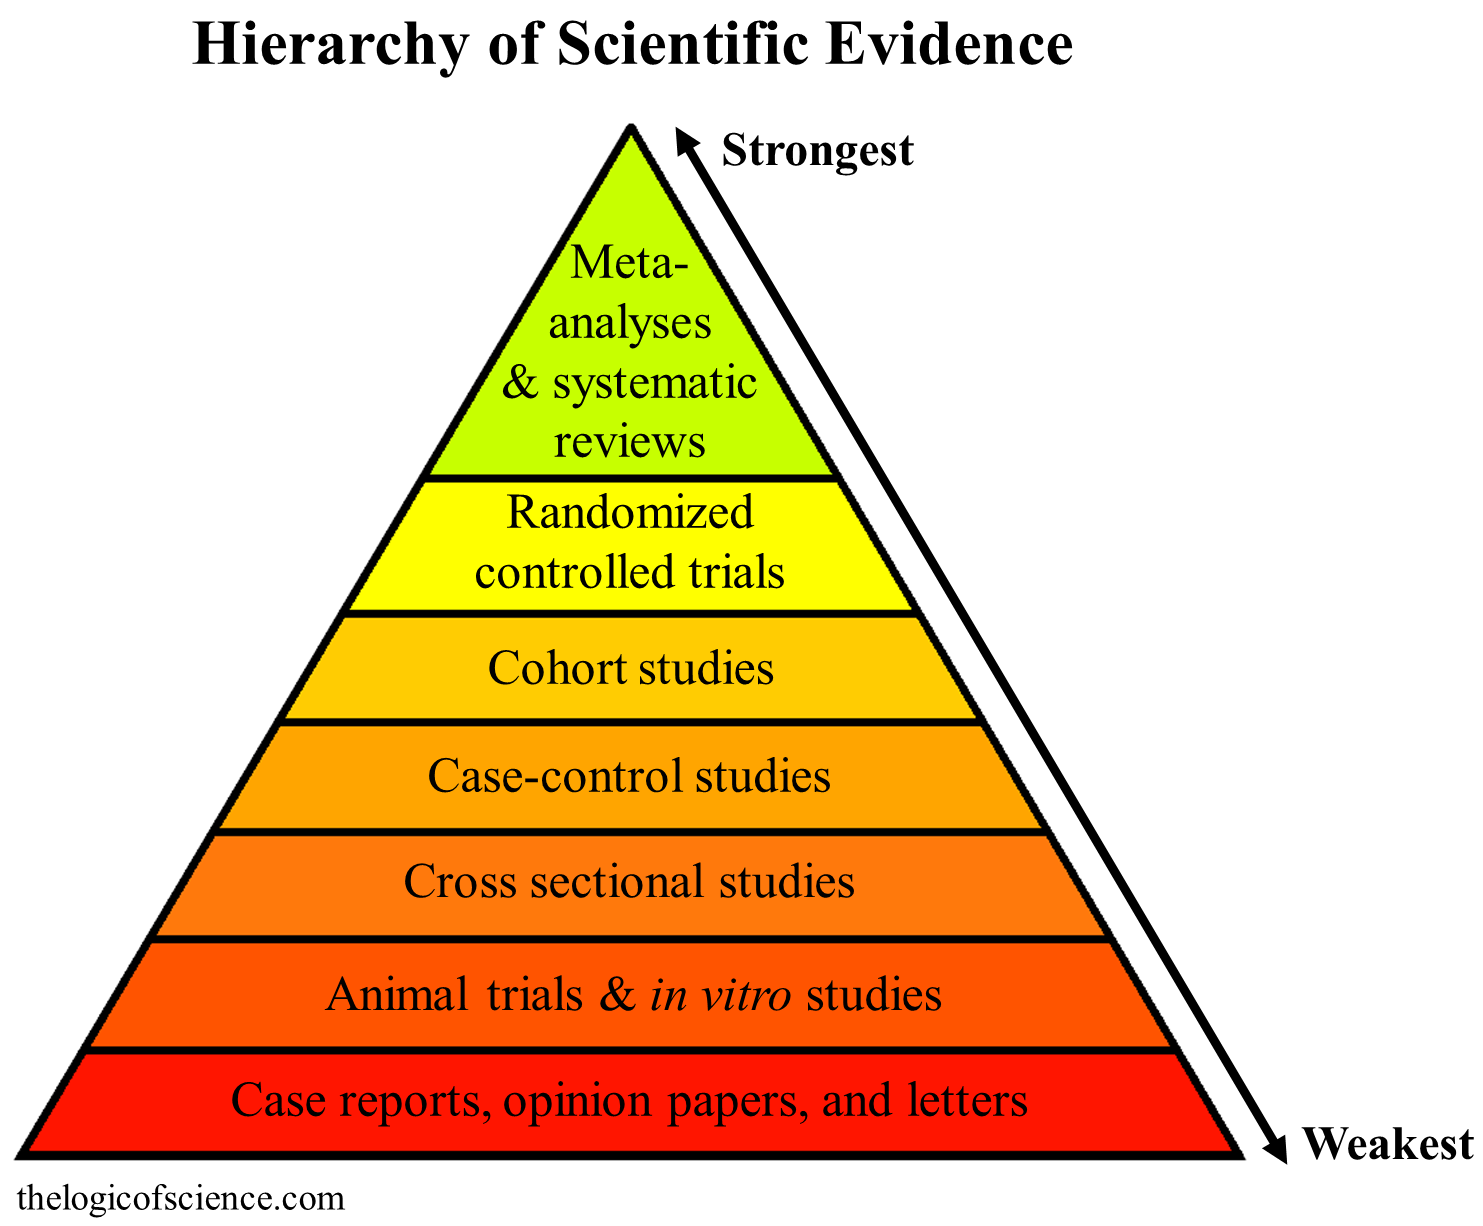
\includegraphics[width=0.6\linewidth,height=\textheight,keepaspectratio]{Hierarchy_of_Evidence.png}
\end{frame}

\begin{frame}{Types of References to Use}
\phantomsection\label{types-of-references-to-use}
\begin{itemize}
\tightlist
\item
  Non-academic articles

  \begin{itemize}
  \tightlist
  \item
    Online research briefs (e.g., Pew Research Center)
  \item
    Mainly used in hook of introduction
  \end{itemize}
\item
  Peer-reviewed articles/conference proceedings

  \begin{itemize}
  \tightlist
  \item
    Empirical research
  \item
    Systematic Reviews/Scoping Reviews/Meta-Analyses
  \end{itemize}
\end{itemize}
\end{frame}

\begin{frame}{Find Research Topic}
\phantomsection\label{find-research-topic}
\begin{itemize}
\item
  Central idea for your research
\item
  Should be researched if

  \begin{itemize}
  \tightlist
  \item
    There is a gap in the literature
  \item
    You have access to data that would answer the topic
  \item
    Advances your academic career
  \end{itemize}
\end{itemize}
\end{frame}

\begin{frame}{Point of the Lit Review}
\phantomsection\label{point-of-the-lit-review}
\begin{itemize}
\item
  Provides a framework showing importance of this research
\item
  You build your argument with supporting or contradicting findings
\item
  Helps solidify your research topic when identifying the gap(s) in the
  literature
\end{itemize}
\end{frame}

\begin{frame}{Literature Maps}
\phantomsection\label{literature-maps}
\begin{itemize}
\tightlist
\item
  Map out how your literature will support your argument

  \begin{itemize}
  \tightlist
  \item
    Create categories to organize your paper into
  \item
    Google \href{https://sites.google.com/view/notebook-lm}{NotebookLM}
  \end{itemize}
\item
  Thinking like this can help with the writing process (when we get
  there)
\end{itemize}
\end{frame}

\begin{frame}{How to read articles}
\phantomsection\label{how-to-read-articles}
\begin{itemize}
\item
  If using AI, go ahead and use that for your initial search
\item
  Read \textbf{abstracts only} the first time through
\item
  Save articles you think may be useful
\item
  Then you can read the articles
\end{itemize}
\end{frame}

\begin{frame}{Abstracts}
\phantomsection\label{abstracts}
\begin{itemize}
\tightlist
\item
\end{itemize}
\end{frame}

\begin{frame}{Introduction}
\phantomsection\label{introduction}
\begin{itemize}
\tightlist
\item
\end{itemize}
\end{frame}

\begin{frame}{Methods}
\phantomsection\label{methods}
\begin{itemize}
\tightlist
\item
\end{itemize}
\end{frame}

\begin{frame}{Results}
\phantomsection\label{results}
\begin{itemize}
\tightlist
\item
\end{itemize}
\end{frame}

\begin{frame}{Discussion/Conclusion}
\phantomsection\label{discussionconclusion}
\begin{itemize}
\tightlist
\item
\end{itemize}
\end{frame}

\begin{frame}{Future Studies/Limitations}
\phantomsection\label{future-studieslimitations}
\begin{itemize}
\tightlist
\item
\end{itemize}
\end{frame}

\begin{frame}{Get an Article}
\phantomsection\label{get-an-article}
\begin{itemize}
\tightlist
\item
\end{itemize}
\end{frame}

\begin{frame}{Annotated Bibliographies}
\phantomsection\label{annotated-bibliographies}
\begin{itemize}
\tightlist
\item
  Different philosophies of how to create annotated bibliographies

  \begin{itemize}
  \tightlist
  \item
    Short paragraphs with all information (\textasciitilde150 words)

    \begin{itemize}
    \tightlist
    \item
      Feels like another abstract
    \end{itemize}
  \end{itemize}
\item
  Spreadsheets
\end{itemize}
\end{frame}

\begin{frame}{Example}
\phantomsection\label{example}
\begin{itemize}
\tightlist
\item
  Make a copy or you could make something similar

  \begin{itemize}
  \tightlist
  \item
    \href{https://docs.google.com/spreadsheets/d/1plQjbtrMaPI9DM4vQAvvtYT2diX3pFjHXNdHUDxG0xE/edit?usp=sharing}{Link
    here for example spreadsheet}
  \end{itemize}
\item
  If you would like to use a document instead

  \begin{itemize}
  \tightlist
  \item
    \href{https://docs.google.com/document/d/13HKVF_CSMAKfT0NoHcd5H4DejZu19BxKZua_tgHF2Lo/edit?usp=sharing}{Link
    here for example document}
  \end{itemize}
\end{itemize}
\end{frame}




\end{document}
